%% ECON 282E -- Session 7, Deck A4: Architecture as a Constraint on W
%% Source: Feng & Miao, "AI for Economists" (Book1), ch.9 section 9.6
%% ("Specialized architectures"), figures fig:cnn_vs_fc, fig:cnn_pipeline,
%% fig:rnn_vs_fc, fig:gnn_vs_fc and table tab:architecture_choice.  The three
%% comparison figures are TikZ in the source and are carried over with their
%% construction intact; captions and labels are rewritten in English.
%% Numbers from tools/figures/s07_numbers.json, key "param_count".

%% ECON 282E -- Foundations of Macroeconomics (UC Riverside, Fall 2026)
%% Shared Beamer preamble for every deck in slides/S01 ... slides/S10.
%%
%% Usage (a deck lives in slides/S0X/ and is compiled from that folder):
%%   %% ECON 282E -- Foundations of Macroeconomics (UC Riverside, Fall 2026)
%% Shared Beamer preamble for every deck in slides/S01 ... slides/S10.
%%
%% Usage (a deck lives in slides/S0X/ and is compiled from that folder):
%%   %% ECON 282E -- Foundations of Macroeconomics (UC Riverside, Fall 2026)
%% Shared Beamer preamble for every deck in slides/S01 ... slides/S10.
%%
%% Usage (a deck lives in slides/S0X/ and is compiled from that folder):
%%   \input{../preamble/course_preamble.tex}
%%   \decktitle{1}{A1}{Who I Am \& Why This Course}{September 24, 2026}
%%   \begin{document}
%%   \makedecktitle
%%   ...
%%
%% Adapted from Courses/AI-ECON-2026/source/shared_preamble.tex (Metropolis theme,
%% concept/caution/example/takeaway boxes, \sectiondivider). Changes for this course:
%%   * course title block (\decktitle / \makedecktitle) instead of \makebeamertitle
%%   * \zh{...} typesets Chinese (book titles) under pdflatex via CJKutf8
%%   * researchbox for the "Research in the wild" frames
%%   * section pages off; TikZ libraries and the course map loaded here
%% Build with pdflatex only (two passes); tools/build_slides.py does this for you.

\documentclass[10pt,english,aspectratio=169]{beamer}

\usepackage[T1]{fontenc}
\usepackage{textcomp}
\usepackage[utf8]{inputenc}
\usepackage{babel}
\usepackage{CJKutf8}

\usepackage{amsmath, amssymb, amsthm, graphicx}
\usepackage{booktabs, multirow, tabularx}
\usepackage{tikz}
\usetikzlibrary{positioning,arrows.meta,shapes,calc,fit,backgrounds}
\usepackage{pgfplots}
\pgfplotsset{compat=1.16}
\usepackage[most]{tcolorbox}
\tcbuselibrary{skins, breakable}
\usepackage{listings}
\usepackage{xcolor}

\lstset{
  basicstyle=\ttfamily\small,
  keywordstyle=\color{blue!80!black}\bfseries,
  commentstyle=\color{green!50!black}\itshape,
  stringstyle=\color{orange!80!black},
  backgroundcolor=\color{gray!8},
  frame=single,
  rulecolor=\color{gray!40},
  breaklines=true,
  showstringspaces=false,
  numbers=none,
}

\usetheme{metropolis}
\usefonttheme{professionalfonts}
\metroset{sectionpage=none}

\definecolor{LightGray}{RGB}{230,230,230}
\definecolor{RedTitle}{RGB}{0,0,200}
\definecolor{VeryLightGray}{RGB}{245,245,245}
\definecolor{DarkText}{RGB}{0,0,0}
\definecolor{UCRBlue}{RGB}{0,45,106}
\definecolor{UCRGold}{RGB}{241,171,0}

% Stage colours of the course arc (used by the course map and elsewhere)
\colorlet{StageTrunk}{blue!12}
\colorlet{StageBranch}{cyan!14}
\colorlet{StageMachine}{gray!18}
\colorlet{StageWall}{red!14}
\colorlet{StageTools}{orange!20}
\colorlet{StageData}{green!16}
\colorlet{StageAgents}{violet!14}

\hypersetup{bookmarks=false,breaklinks=true,pdfborder={0 0 0},colorlinks=true,
  linkcolor=DarkText,urlcolor=RedTitle}

\setbeamercolor{background canvas}{bg=white}
\setbeamercolor{title}{fg=RedTitle}
\setbeamercolor{frametitle}{bg=VeryLightGray,fg=DarkText}
\setbeamercolor{normal text}{fg=DarkText}
\setbeamercolor{alerted text}{fg=RedTitle}
\setbeamersize{text margin left=5mm, text margin right=5mm}
\addtobeamertemplate{frametitle}{}{\vspace{-0.5em}}

\setbeamertemplate{navigation symbols}{}
\setbeamertemplate{footline}{%
  \hspace{5mm}{\usebeamerfont{page number in head/foot}\color{black!45}%
  ECON 282E \,$\cdot$\, \insertshortdeck}\hfill%
  \usebeamercolor[fg]{page number in head/foot}%
  \usebeamerfont{page number in head/foot}%
  \insertframenumber\,/\,\inserttotalframenumber\kern1em\vskip2pt%
}

% ---------------------------------------------------------------------------
% Chinese text under pdflatex (book titles etc.)
\newcommand{\zh}[1]{\begin{CJK*}{UTF8}{gbsn}#1\end{CJK*}}

% ---------------------------------------------------------------------------
% Deck title block
%   \decktitle{session}{deck id}{title}{date}
\newcommand{\insertshortdeck}{}
\newcommand{\decksession}{}
\newcommand{\deckid}{}
\newcommand{\decktitletext}{}
\newcommand{\deckdate}{}
\newcommand{\decktitle}[4]{%
  \renewcommand{\decksession}{#1}%
  \renewcommand{\deckid}{#2}%
  \renewcommand{\decktitletext}{#3}%
  \renewcommand{\deckdate}{#4}%
  \renewcommand{\insertshortdeck}{Session #1 \,$\cdot$\, Deck #1.#2}%
  \title{#3}%
  \author{Zhigang Feng}%
  \date{#4}%
}
\newcommand{\makedecktitle}{%
  \begin{frame}[plain,noframenumbering]
    \begin{tikzpicture}[remember picture,overlay]
      \fill[UCRBlue] (current page.north west) rectangle ([yshift=-0.55cm]current page.north east);
      \fill[UCRGold] ([yshift=-0.55cm]current page.north west) rectangle ([yshift=-0.62cm]current page.north east);
      \node[anchor=west, text=white, font=\small\bfseries] at ([xshift=5mm,yshift=-0.275cm]current page.north west)
        {ECON 282E \,$\cdot$\, Foundations of Macroeconomics};
      \node[anchor=east, text=white, font=\small] at ([xshift=-5mm,yshift=-0.275cm]current page.north east)
        {UC Riverside \,$\cdot$\, Fall 2026};
    \end{tikzpicture}
    \vspace*{1.1cm}
    {\usebeamerfont{title}\color{black!55}\large Session \decksession\ \,$\cdot$\, Deck \decksession.\deckid\par}
    \vspace{0.25cm}
    {\usebeamerfont{title}\color{RedTitle}\LARGE\bfseries \decktitletext\par}
    \vspace{0.7cm}
    {\large Zhigang Feng\par}
    \vspace{0.15cm}
    {\color{black!65}\deckdate\par}
    \vfill
    {\footnotesize\itshape\color{black!55}Build it on paper $\;\to\;$ solve it on the machine $\;\to\;$ push it to the frontier with AI\par}
  \end{frame}}

% ---------------------------------------------------------------------------
% Section divider (plain frame, not counted)
\newcommand{\sectiondivider}[2]{%
\begin{frame}[plain,noframenumbering]
\begin{center}
\vfill
{\Large\textbf{#1}\par}
\vspace{0.35cm}
{\normalsize #2\par}
\vfill
\end{center}
\end{frame}
}

% ---------------------------------------------------------------------------
% Boxes
\newtcolorbox{conceptbox}[1][]{colback=blue!3, colframe=RedTitle!55, boxrule=0.35mm,
  arc=1mm, left=2mm, right=2mm, top=1mm, bottom=1mm, #1}
\newtcolorbox{cautionbox}[1][]{colback=red!3, colframe=red!50!black, boxrule=0.35mm,
  arc=1mm, left=2mm, right=2mm, top=1mm, bottom=1mm, #1}
\newtcolorbox{examplebox}[1][]{colback=green!3, colframe=green!45!black, boxrule=0.35mm,
  arc=1mm, left=2mm, right=2mm, top=1mm, bottom=1mm, #1}
\newtcolorbox{takeawaybox}[1][]{colback=VeryLightGray, colframe=RedTitle!55, boxrule=0.35mm,
  arc=1mm, left=2mm, right=2mm, top=1mm, bottom=1mm, #1}
\newtcolorbox{researchbox}[1][]{enhanced, colback=violet!4, colframe=violet!60!black,
  boxrule=0.35mm, arc=1mm, left=2mm, right=2mm, top=1mm, bottom=1mm,
  fonttitle=\bfseries\small, title={Research in the wild}, #1}

\newcommand{\compacttables}{\renewcommand{\arraystretch}{1.15}}
\newcommand{\src}[1]{{\tiny\color{black!55}#1}}

% ---------------------------------------------------------------------------
\input{../preamble/course_map.tex}

%%   \decktitle{1}{A1}{Who I Am \& Why This Course}{September 24, 2026}
%%   \begin{document}
%%   \makedecktitle
%%   ...
%%
%% Adapted from Courses/AI-ECON-2026/source/shared_preamble.tex (Metropolis theme,
%% concept/caution/example/takeaway boxes, \sectiondivider). Changes for this course:
%%   * course title block (\decktitle / \makedecktitle) instead of \makebeamertitle
%%   * \zh{...} typesets Chinese (book titles) under pdflatex via CJKutf8
%%   * researchbox for the "Research in the wild" frames
%%   * section pages off; TikZ libraries and the course map loaded here
%% Build with pdflatex only (two passes); tools/build_slides.py does this for you.

\documentclass[10pt,english,aspectratio=169]{beamer}

\usepackage[T1]{fontenc}
\usepackage{textcomp}
\usepackage[utf8]{inputenc}
\usepackage{babel}
\usepackage{CJKutf8}

\usepackage{amsmath, amssymb, amsthm, graphicx}
\usepackage{booktabs, multirow, tabularx}
\usepackage{tikz}
\usetikzlibrary{positioning,arrows.meta,shapes,calc,fit,backgrounds}
\usepackage{pgfplots}
\pgfplotsset{compat=1.16}
\usepackage[most]{tcolorbox}
\tcbuselibrary{skins, breakable}
\usepackage{listings}
\usepackage{xcolor}

\lstset{
  basicstyle=\ttfamily\small,
  keywordstyle=\color{blue!80!black}\bfseries,
  commentstyle=\color{green!50!black}\itshape,
  stringstyle=\color{orange!80!black},
  backgroundcolor=\color{gray!8},
  frame=single,
  rulecolor=\color{gray!40},
  breaklines=true,
  showstringspaces=false,
  numbers=none,
}

\usetheme{metropolis}
\usefonttheme{professionalfonts}
\metroset{sectionpage=none}

\definecolor{LightGray}{RGB}{230,230,230}
\definecolor{RedTitle}{RGB}{0,0,200}
\definecolor{VeryLightGray}{RGB}{245,245,245}
\definecolor{DarkText}{RGB}{0,0,0}
\definecolor{UCRBlue}{RGB}{0,45,106}
\definecolor{UCRGold}{RGB}{241,171,0}

% Stage colours of the course arc (used by the course map and elsewhere)
\colorlet{StageTrunk}{blue!12}
\colorlet{StageBranch}{cyan!14}
\colorlet{StageMachine}{gray!18}
\colorlet{StageWall}{red!14}
\colorlet{StageTools}{orange!20}
\colorlet{StageData}{green!16}
\colorlet{StageAgents}{violet!14}

\hypersetup{bookmarks=false,breaklinks=true,pdfborder={0 0 0},colorlinks=true,
  linkcolor=DarkText,urlcolor=RedTitle}

\setbeamercolor{background canvas}{bg=white}
\setbeamercolor{title}{fg=RedTitle}
\setbeamercolor{frametitle}{bg=VeryLightGray,fg=DarkText}
\setbeamercolor{normal text}{fg=DarkText}
\setbeamercolor{alerted text}{fg=RedTitle}
\setbeamersize{text margin left=5mm, text margin right=5mm}
\addtobeamertemplate{frametitle}{}{\vspace{-0.5em}}

\setbeamertemplate{navigation symbols}{}
\setbeamertemplate{footline}{%
  \hspace{5mm}{\usebeamerfont{page number in head/foot}\color{black!45}%
  ECON 282E \,$\cdot$\, \insertshortdeck}\hfill%
  \usebeamercolor[fg]{page number in head/foot}%
  \usebeamerfont{page number in head/foot}%
  \insertframenumber\,/\,\inserttotalframenumber\kern1em\vskip2pt%
}

% ---------------------------------------------------------------------------
% Chinese text under pdflatex (book titles etc.)
\newcommand{\zh}[1]{\begin{CJK*}{UTF8}{gbsn}#1\end{CJK*}}

% ---------------------------------------------------------------------------
% Deck title block
%   \decktitle{session}{deck id}{title}{date}
\newcommand{\insertshortdeck}{}
\newcommand{\decksession}{}
\newcommand{\deckid}{}
\newcommand{\decktitletext}{}
\newcommand{\deckdate}{}
\newcommand{\decktitle}[4]{%
  \renewcommand{\decksession}{#1}%
  \renewcommand{\deckid}{#2}%
  \renewcommand{\decktitletext}{#3}%
  \renewcommand{\deckdate}{#4}%
  \renewcommand{\insertshortdeck}{Session #1 \,$\cdot$\, Deck #1.#2}%
  \title{#3}%
  \author{Zhigang Feng}%
  \date{#4}%
}
\newcommand{\makedecktitle}{%
  \begin{frame}[plain,noframenumbering]
    \begin{tikzpicture}[remember picture,overlay]
      \fill[UCRBlue] (current page.north west) rectangle ([yshift=-0.55cm]current page.north east);
      \fill[UCRGold] ([yshift=-0.55cm]current page.north west) rectangle ([yshift=-0.62cm]current page.north east);
      \node[anchor=west, text=white, font=\small\bfseries] at ([xshift=5mm,yshift=-0.275cm]current page.north west)
        {ECON 282E \,$\cdot$\, Foundations of Macroeconomics};
      \node[anchor=east, text=white, font=\small] at ([xshift=-5mm,yshift=-0.275cm]current page.north east)
        {UC Riverside \,$\cdot$\, Fall 2026};
    \end{tikzpicture}
    \vspace*{1.1cm}
    {\usebeamerfont{title}\color{black!55}\large Session \decksession\ \,$\cdot$\, Deck \decksession.\deckid\par}
    \vspace{0.25cm}
    {\usebeamerfont{title}\color{RedTitle}\LARGE\bfseries \decktitletext\par}
    \vspace{0.7cm}
    {\large Zhigang Feng\par}
    \vspace{0.15cm}
    {\color{black!65}\deckdate\par}
    \vfill
    {\footnotesize\itshape\color{black!55}Build it on paper $\;\to\;$ solve it on the machine $\;\to\;$ push it to the frontier with AI\par}
  \end{frame}}

% ---------------------------------------------------------------------------
% Section divider (plain frame, not counted)
\newcommand{\sectiondivider}[2]{%
\begin{frame}[plain,noframenumbering]
\begin{center}
\vfill
{\Large\textbf{#1}\par}
\vspace{0.35cm}
{\normalsize #2\par}
\vfill
\end{center}
\end{frame}
}

% ---------------------------------------------------------------------------
% Boxes
\newtcolorbox{conceptbox}[1][]{colback=blue!3, colframe=RedTitle!55, boxrule=0.35mm,
  arc=1mm, left=2mm, right=2mm, top=1mm, bottom=1mm, #1}
\newtcolorbox{cautionbox}[1][]{colback=red!3, colframe=red!50!black, boxrule=0.35mm,
  arc=1mm, left=2mm, right=2mm, top=1mm, bottom=1mm, #1}
\newtcolorbox{examplebox}[1][]{colback=green!3, colframe=green!45!black, boxrule=0.35mm,
  arc=1mm, left=2mm, right=2mm, top=1mm, bottom=1mm, #1}
\newtcolorbox{takeawaybox}[1][]{colback=VeryLightGray, colframe=RedTitle!55, boxrule=0.35mm,
  arc=1mm, left=2mm, right=2mm, top=1mm, bottom=1mm, #1}
\newtcolorbox{researchbox}[1][]{enhanced, colback=violet!4, colframe=violet!60!black,
  boxrule=0.35mm, arc=1mm, left=2mm, right=2mm, top=1mm, bottom=1mm,
  fonttitle=\bfseries\small, title={Research in the wild}, #1}

\newcommand{\compacttables}{\renewcommand{\arraystretch}{1.15}}
\newcommand{\src}[1]{{\tiny\color{black!55}#1}}

% ---------------------------------------------------------------------------
%% Course map: the recurring "you are here" slide for ECON 282E.
%% Loaded by course_preamble.tex. Pattern follows AI-ECON-2026 lec01_map.tex, but the map
%% shows the whole ten-session course rather than one lecture.
%%
%%   \CourseMap{s}{label}   s = 1..10 highlights session s and prints "you are here: label"
%%                          (e.g. \CourseMap{1}{1.A2}); earlier sessions get a check mark.
%%   \CourseMap{0}{}        full overview, nothing highlighted.
%%
%% Note: TikZ option lists are comma-split before TeX conditionals run, so every \ifnum
%% below sits outside [...] option lists.

\newcommand{\CourseMap}[2]{%
\begin{center}
\begin{tikzpicture}[
    sess/.style={rectangle, rounded corners=2pt, draw=black!45, minimum width=1.34cm,
        minimum height=1.12cm, text width=1.26cm, align=center, inner sep=1pt},
    stage/.style={font=\tiny\bfseries, text=black!70},
]
  \foreach \i/\d/\t/\c in {%
      1/Sep 24/Intro \\ Growth/StageTrunk,
      2/Oct 1/HA $\cdot$ OLG \\ Policy/StageBranch,
      3/Oct 8/Num.\ DP \\ Python/StageMachine,
      4/Oct 15/Numerics \\ I/StageMachine,
      5/Oct 22/Numerics \\ II/StageMachine,
      6/Oct 29/The wall \\ \textbf{Midterm}/StageWall,
      7/Nov 5/ML \\ Deep nets/StageTools,
      8/Nov 12/RL \\ HA $+$ DL/StageTools,
      9/Nov 19/Text \\ LLMs/StageData,
      10/Dec 3/Agents \\ \textbf{Projects}/StageAgents} {
    \node[sess, fill=\c] (n\i) at ({1.46*(\i-1)}, 0)
      {{\scriptsize\bfseries S\i}\\[-1pt]{\tiny\color{black!60}\d}\\[1pt]{\tiny \t}};
    \ifnum\i<#1
      \node[font=\scriptsize, text=green!45!black] at ([xshift=-2.5mm,yshift=-2.2mm]n\i.north east) {$\checkmark$};
    \fi
    \ifnum\i=#1
      \draw[RedTitle, very thick, rounded corners=2pt]
        ([xshift=-0.6mm,yshift=-0.6mm]n\i.south west) rectangle ([xshift=0.6mm,yshift=0.6mm]n\i.north east);
      % keep the label inside the picture at both ends of the row
      \ifnum\i<3
        \node[font=\scriptsize\bfseries, text=RedTitle, anchor=south west] at ([yshift=1.2mm]n\i.north west)
          {$\blacktriangledown$\,you are here: #2};
      \else\ifnum\i>8
        \node[font=\scriptsize\bfseries, text=RedTitle, anchor=south east] at ([yshift=1.2mm]n\i.north east)
          {you are here: #2\,$\blacktriangledown$};
      \else
        \node[font=\scriptsize\bfseries, text=RedTitle, anchor=south] at ([yshift=1.2mm]n\i.north)
          {you are here: #2\,$\blacktriangledown$};
      \fi\fi
    \fi
  }
  % stage band under the sessions
  \foreach \a/\b/\lab/\c in {1/1/trunk/StageTrunk, 2/2/branches/StageBranch,
      3/5/the machine $\cdot$ classical methods/StageMachine, 6/6/the wall/StageWall,
      7/8/new tools/StageTools, 9/9/new data/StageData, 10/10/colleagues/StageAgents} {
    \fill[\c] ([yshift=-1.5mm]n\a.south west) rectangle ([yshift=-4.6mm]n\b.south east);
    \path ([yshift=-1.5mm]n\a.south west) -- ([yshift=-4.6mm]n\b.south east)
      node[midway, stage] {\lab};
  }
  \node[font=\footnotesize\itshape, text=black!70] at ([yshift=-9.5mm]$(n1.south)!0.5!(n10.south)$)
    {Build it on paper $\;\to\;$ solve it on the machine $\;\to\;$ push it to the frontier with AI};
\end{tikzpicture}
\end{center}
}


%%   \decktitle{1}{A1}{Who I Am \& Why This Course}{September 24, 2026}
%%   \begin{document}
%%   \makedecktitle
%%   ...
%%
%% Adapted from Courses/AI-ECON-2026/source/shared_preamble.tex (Metropolis theme,
%% concept/caution/example/takeaway boxes, \sectiondivider). Changes for this course:
%%   * course title block (\decktitle / \makedecktitle) instead of \makebeamertitle
%%   * \zh{...} typesets Chinese (book titles) under pdflatex via CJKutf8
%%   * researchbox for the "Research in the wild" frames
%%   * section pages off; TikZ libraries and the course map loaded here
%% Build with pdflatex only (two passes); tools/build_slides.py does this for you.

\documentclass[10pt,english,aspectratio=169]{beamer}

\usepackage[T1]{fontenc}
\usepackage{textcomp}
\usepackage[utf8]{inputenc}
\usepackage{babel}
\usepackage{CJKutf8}

\usepackage{amsmath, amssymb, amsthm, graphicx}
\usepackage{booktabs, multirow, tabularx}
\usepackage{tikz}
\usetikzlibrary{positioning,arrows.meta,shapes,calc,fit,backgrounds}
\usepackage{pgfplots}
\pgfplotsset{compat=1.16}
\usepackage[most]{tcolorbox}
\tcbuselibrary{skins, breakable}
\usepackage{listings}
\usepackage{xcolor}

\lstset{
  basicstyle=\ttfamily\small,
  keywordstyle=\color{blue!80!black}\bfseries,
  commentstyle=\color{green!50!black}\itshape,
  stringstyle=\color{orange!80!black},
  backgroundcolor=\color{gray!8},
  frame=single,
  rulecolor=\color{gray!40},
  breaklines=true,
  showstringspaces=false,
  numbers=none,
}

\usetheme{metropolis}
\usefonttheme{professionalfonts}
\metroset{sectionpage=none}

\definecolor{LightGray}{RGB}{230,230,230}
\definecolor{RedTitle}{RGB}{0,0,200}
\definecolor{VeryLightGray}{RGB}{245,245,245}
\definecolor{DarkText}{RGB}{0,0,0}
\definecolor{UCRBlue}{RGB}{0,45,106}
\definecolor{UCRGold}{RGB}{241,171,0}

% Stage colours of the course arc (used by the course map and elsewhere)
\colorlet{StageTrunk}{blue!12}
\colorlet{StageBranch}{cyan!14}
\colorlet{StageMachine}{gray!18}
\colorlet{StageWall}{red!14}
\colorlet{StageTools}{orange!20}
\colorlet{StageData}{green!16}
\colorlet{StageAgents}{violet!14}

\hypersetup{bookmarks=false,breaklinks=true,pdfborder={0 0 0},colorlinks=true,
  linkcolor=DarkText,urlcolor=RedTitle}

\setbeamercolor{background canvas}{bg=white}
\setbeamercolor{title}{fg=RedTitle}
\setbeamercolor{frametitle}{bg=VeryLightGray,fg=DarkText}
\setbeamercolor{normal text}{fg=DarkText}
\setbeamercolor{alerted text}{fg=RedTitle}
\setbeamersize{text margin left=5mm, text margin right=5mm}
\addtobeamertemplate{frametitle}{}{\vspace{-0.5em}}

\setbeamertemplate{navigation symbols}{}
\setbeamertemplate{footline}{%
  \hspace{5mm}{\usebeamerfont{page number in head/foot}\color{black!45}%
  ECON 282E \,$\cdot$\, \insertshortdeck}\hfill%
  \usebeamercolor[fg]{page number in head/foot}%
  \usebeamerfont{page number in head/foot}%
  \insertframenumber\,/\,\inserttotalframenumber\kern1em\vskip2pt%
}

% ---------------------------------------------------------------------------
% Chinese text under pdflatex (book titles etc.)
\newcommand{\zh}[1]{\begin{CJK*}{UTF8}{gbsn}#1\end{CJK*}}

% ---------------------------------------------------------------------------
% Deck title block
%   \decktitle{session}{deck id}{title}{date}
\newcommand{\insertshortdeck}{}
\newcommand{\decksession}{}
\newcommand{\deckid}{}
\newcommand{\decktitletext}{}
\newcommand{\deckdate}{}
\newcommand{\decktitle}[4]{%
  \renewcommand{\decksession}{#1}%
  \renewcommand{\deckid}{#2}%
  \renewcommand{\decktitletext}{#3}%
  \renewcommand{\deckdate}{#4}%
  \renewcommand{\insertshortdeck}{Session #1 \,$\cdot$\, Deck #1.#2}%
  \title{#3}%
  \author{Zhigang Feng}%
  \date{#4}%
}
\newcommand{\makedecktitle}{%
  \begin{frame}[plain,noframenumbering]
    \begin{tikzpicture}[remember picture,overlay]
      \fill[UCRBlue] (current page.north west) rectangle ([yshift=-0.55cm]current page.north east);
      \fill[UCRGold] ([yshift=-0.55cm]current page.north west) rectangle ([yshift=-0.62cm]current page.north east);
      \node[anchor=west, text=white, font=\small\bfseries] at ([xshift=5mm,yshift=-0.275cm]current page.north west)
        {ECON 282E \,$\cdot$\, Foundations of Macroeconomics};
      \node[anchor=east, text=white, font=\small] at ([xshift=-5mm,yshift=-0.275cm]current page.north east)
        {UC Riverside \,$\cdot$\, Fall 2026};
    \end{tikzpicture}
    \vspace*{1.1cm}
    {\usebeamerfont{title}\color{black!55}\large Session \decksession\ \,$\cdot$\, Deck \decksession.\deckid\par}
    \vspace{0.25cm}
    {\usebeamerfont{title}\color{RedTitle}\LARGE\bfseries \decktitletext\par}
    \vspace{0.7cm}
    {\large Zhigang Feng\par}
    \vspace{0.15cm}
    {\color{black!65}\deckdate\par}
    \vfill
    {\footnotesize\itshape\color{black!55}Build it on paper $\;\to\;$ solve it on the machine $\;\to\;$ push it to the frontier with AI\par}
  \end{frame}}

% ---------------------------------------------------------------------------
% Section divider (plain frame, not counted)
\newcommand{\sectiondivider}[2]{%
\begin{frame}[plain,noframenumbering]
\begin{center}
\vfill
{\Large\textbf{#1}\par}
\vspace{0.35cm}
{\normalsize #2\par}
\vfill
\end{center}
\end{frame}
}

% ---------------------------------------------------------------------------
% Boxes
\newtcolorbox{conceptbox}[1][]{colback=blue!3, colframe=RedTitle!55, boxrule=0.35mm,
  arc=1mm, left=2mm, right=2mm, top=1mm, bottom=1mm, #1}
\newtcolorbox{cautionbox}[1][]{colback=red!3, colframe=red!50!black, boxrule=0.35mm,
  arc=1mm, left=2mm, right=2mm, top=1mm, bottom=1mm, #1}
\newtcolorbox{examplebox}[1][]{colback=green!3, colframe=green!45!black, boxrule=0.35mm,
  arc=1mm, left=2mm, right=2mm, top=1mm, bottom=1mm, #1}
\newtcolorbox{takeawaybox}[1][]{colback=VeryLightGray, colframe=RedTitle!55, boxrule=0.35mm,
  arc=1mm, left=2mm, right=2mm, top=1mm, bottom=1mm, #1}
\newtcolorbox{researchbox}[1][]{enhanced, colback=violet!4, colframe=violet!60!black,
  boxrule=0.35mm, arc=1mm, left=2mm, right=2mm, top=1mm, bottom=1mm,
  fonttitle=\bfseries\small, title={Research in the wild}, #1}

\newcommand{\compacttables}{\renewcommand{\arraystretch}{1.15}}
\newcommand{\src}[1]{{\tiny\color{black!55}#1}}

% ---------------------------------------------------------------------------
%% Course map: the recurring "you are here" slide for ECON 282E.
%% Loaded by course_preamble.tex. Pattern follows AI-ECON-2026 lec01_map.tex, but the map
%% shows the whole ten-session course rather than one lecture.
%%
%%   \CourseMap{s}{label}   s = 1..10 highlights session s and prints "you are here: label"
%%                          (e.g. \CourseMap{1}{1.A2}); earlier sessions get a check mark.
%%   \CourseMap{0}{}        full overview, nothing highlighted.
%%
%% Note: TikZ option lists are comma-split before TeX conditionals run, so every \ifnum
%% below sits outside [...] option lists.

\newcommand{\CourseMap}[2]{%
\begin{center}
\begin{tikzpicture}[
    sess/.style={rectangle, rounded corners=2pt, draw=black!45, minimum width=1.34cm,
        minimum height=1.12cm, text width=1.26cm, align=center, inner sep=1pt},
    stage/.style={font=\tiny\bfseries, text=black!70},
]
  \foreach \i/\d/\t/\c in {%
      1/Sep 24/Intro \\ Growth/StageTrunk,
      2/Oct 1/HA $\cdot$ OLG \\ Policy/StageBranch,
      3/Oct 8/Num.\ DP \\ Python/StageMachine,
      4/Oct 15/Numerics \\ I/StageMachine,
      5/Oct 22/Numerics \\ II/StageMachine,
      6/Oct 29/The wall \\ \textbf{Midterm}/StageWall,
      7/Nov 5/ML \\ Deep nets/StageTools,
      8/Nov 12/RL \\ HA $+$ DL/StageTools,
      9/Nov 19/Text \\ LLMs/StageData,
      10/Dec 3/Agents \\ \textbf{Projects}/StageAgents} {
    \node[sess, fill=\c] (n\i) at ({1.46*(\i-1)}, 0)
      {{\scriptsize\bfseries S\i}\\[-1pt]{\tiny\color{black!60}\d}\\[1pt]{\tiny \t}};
    \ifnum\i<#1
      \node[font=\scriptsize, text=green!45!black] at ([xshift=-2.5mm,yshift=-2.2mm]n\i.north east) {$\checkmark$};
    \fi
    \ifnum\i=#1
      \draw[RedTitle, very thick, rounded corners=2pt]
        ([xshift=-0.6mm,yshift=-0.6mm]n\i.south west) rectangle ([xshift=0.6mm,yshift=0.6mm]n\i.north east);
      % keep the label inside the picture at both ends of the row
      \ifnum\i<3
        \node[font=\scriptsize\bfseries, text=RedTitle, anchor=south west] at ([yshift=1.2mm]n\i.north west)
          {$\blacktriangledown$\,you are here: #2};
      \else\ifnum\i>8
        \node[font=\scriptsize\bfseries, text=RedTitle, anchor=south east] at ([yshift=1.2mm]n\i.north east)
          {you are here: #2\,$\blacktriangledown$};
      \else
        \node[font=\scriptsize\bfseries, text=RedTitle, anchor=south] at ([yshift=1.2mm]n\i.north)
          {you are here: #2\,$\blacktriangledown$};
      \fi\fi
    \fi
  }
  % stage band under the sessions
  \foreach \a/\b/\lab/\c in {1/1/trunk/StageTrunk, 2/2/branches/StageBranch,
      3/5/the machine $\cdot$ classical methods/StageMachine, 6/6/the wall/StageWall,
      7/8/new tools/StageTools, 9/9/new data/StageData, 10/10/colleagues/StageAgents} {
    \fill[\c] ([yshift=-1.5mm]n\a.south west) rectangle ([yshift=-4.6mm]n\b.south east);
    \path ([yshift=-1.5mm]n\a.south west) -- ([yshift=-4.6mm]n\b.south east)
      node[midway, stage] {\lab};
  }
  \node[font=\footnotesize\itshape, text=black!70] at ([yshift=-9.5mm]$(n1.south)!0.5!(n10.south)$)
    {Build it on paper $\;\to\;$ solve it on the machine $\;\to\;$ push it to the frontier with AI};
\end{tikzpicture}
\end{center}
}


\graphicspath{{./figures/}}

%% Deck-local: the shared preamble is never edited (its md5 marks every deck stale).
\newcommand{\repo}[2]{\href{https://github.com/vonzhg/Macro-2026Fall/blob/main/#1}{\texttt{#2}}}

\decktitle{7}{A4}{Architecture as a Constraint on $\mathbf{W}$}{Thursday, November 5, 2026}

\begin{document}

\makedecktitle

%=============================================================================
\begin{frame}{Where We Are}
\CourseMap{7}{7.A4}
\vspace{-1mm}
\begin{center}
\small \textbf{Block A:} 7.A1 ML for macroeconomists $\;\cdot\;$ 7.A2 nets as approximators $\;\cdot\;$ 7.A3 training $\;\cdot\;$ \textbf{7.A4} architecture.
\end{center}
\end{frame}

%=============================================================================
\begin{frame}{One Idea, Three Times}
\begin{columns}[T]
\begin{column}{0.55\textwidth}
\small
A feedforward layer is $\sigma(\mathbf{W}\mathbf{x}+\mathbf{b})$ with $\mathbf{W}$ \textbf{dense}: every entry is a free parameter. That is what makes it general --- it assumes nothing about the input --- and it is also what makes it expensive, because anything that could have been written into the structure has to be learned from data instead.
\medskip

Every specialised architecture in this deck is the same layer with a \textbf{constraint on $\mathbf{W}$}:
\begin{itemize}\small\setlength{\itemsep}{1mm}
  \item \textbf{CNN} --- $\mathbf{W}$ sparse \emph{and} repeated;
  \item \textbf{RNN} --- one $\mathbf{W}$ shared across dates;
  \item \textbf{GNN} --- the sparsity pattern follows the adjacency.
\end{itemize}
\end{column}
\begin{column}{0.42\textwidth}
\begin{conceptbox}[title=\textbf{The trade, stated once}]\small
A constraint shrinks the hypothesis space. The \textbf{cost} is that the assumption must be true. The \textbf{return} is fewer parameters, and so fewer observations needed to pin them down.
\end{conceptbox}
\medskip
\begin{takeawaybox}\footnotesize
This is 7.A2's lesson in another key: a network is a basis you do not choose. An \emph{architecture} is the part of the basis you \emph{do} choose.
\end{takeawaybox}
\end{column}
\end{columns}
\vspace{1mm}
\src{Feng \& Miao, \emph{AI for Economists}, ch.~9, ``Specialized architectures''.}
\end{frame}

%=============================================================================
\begin{frame}{Feedforward vs.\ Convolution}
\begin{center}
\resizebox{0.97\textwidth}{!}{%
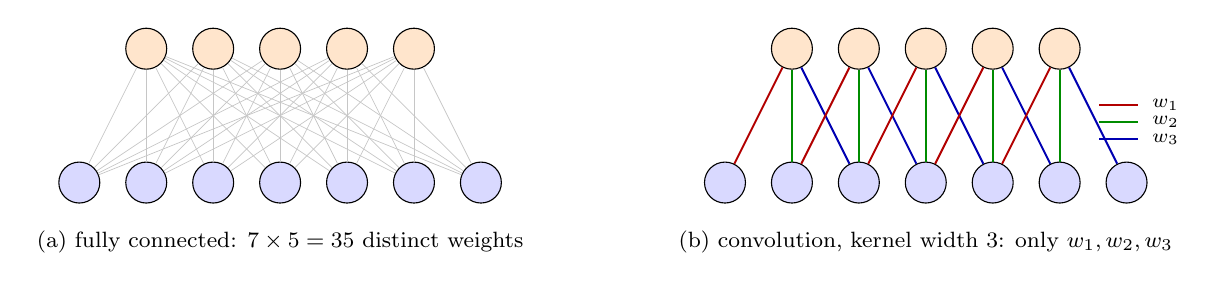
\begin{tikzpicture}[
  every node/.style={font=\small},
  unit/.style={circle, draw, minimum size=0.52cm, inner sep=0pt, font=\scriptsize},
  inp/.style={unit, fill=blue!15},
  outp/.style={unit, fill=orange!20}
]
\begin{scope}
  \foreach \i in {1,...,7} \node[inp] (a\i) at (\i*0.85, 0) {};
  \foreach \j in {1,...,5} \node[outp] (b\j) at (\j*0.85+0.85, 1.7) {};
  \foreach \i in {1,...,7} \foreach \j in {1,...,5}
    \draw[gray!45, line width=0.25pt] (a\i) -- (b\j);
  \node[font=\footnotesize] at (3.4,-0.75) {(a) fully connected: $7\times5=35$ distinct weights};
\end{scope}
\begin{scope}[xshift=8.2cm]
  \foreach \i in {1,...,7} \node[inp] (c\i) at (\i*0.85, 0) {};
  \foreach \j in {1,...,5} \node[outp] (d\j) at (\j*0.85+0.85, 1.7) {};
  \foreach \j in {1,...,5} {
    \pgfmathtruncatemacro{\p}{\j}
    \pgfmathtruncatemacro{\q}{\j+1}
    \pgfmathtruncatemacro{\r}{\j+2}
    \draw[red!70!black,   line width=0.7pt] (c\p) -- (d\j);
    \draw[green!55!black, line width=0.7pt] (c\q) -- (d\j);
    \draw[blue!70!black,  line width=0.7pt] (c\r) -- (d\j);
  }
  \node[font=\footnotesize] at (3.4,-0.75) {(b) convolution, kernel width 3: only $w_1,w_2,w_3$};
  \begin{scope}[shift={(5.6,0.55)}]
    \draw[red!70!black,   line width=0.7pt] (0,0.44) -- (0.5,0.44); \node[right, font=\scriptsize] at (0.55,0.44) {$w_1$};
    \draw[green!55!black, line width=0.7pt] (0,0.22) -- (0.5,0.22); \node[right, font=\scriptsize] at (0.55,0.22) {$w_2$};
    \draw[blue!70!black,  line width=0.7pt] (0,0.00) -- (0.5,0.00); \node[right, font=\scriptsize] at (0.55,0.00) {$w_3$};
  \end{scope}
\end{scope}
\end{tikzpicture}}
\end{center}
\vspace{1mm}
{\footnotesize Seven inputs, five outputs. On the left, 35 lines and 35 free parameters. On the right each output sees only \textbf{three adjacent} inputs (local connection), and lines of the same colour \textbf{share one parameter} (weight sharing): \textbf{three} free parameters in the whole layer.}
\medskip

\begin{takeawaybox}\footnotesize
\textbf{Convolution is not a new operation.} It is a feedforward layer after two constraints --- sparse, and repeated --- are imposed on $\mathbf{W}$.
\end{takeawaybox}
\vspace{1mm}
\src{Feng \& Miao, \emph{AI for Economists}, ch.~9, Fig.~9.9. Ledger \texttt{param\_count.schematic\_1d}. Code: \repo{tools/figures/s07_generate.py}{s07\_generate.py}, \texttt{run\_param\_count}.}
\end{frame}

%=============================================================================
\begin{frame}{What the Constraint Buys, and What It Assumes}
\begin{columns}[T]
\begin{column}{0.54\textwidth}
\small
A $256\times256$ colour image is $196{,}608$ numbers. A dense first layer into 256 units needs about $5\times10^{7}$ weights. Sixty-four $3\times3$ kernels need
\[
  64\times(3\times3\times3+1)=1{,}792,
\]
about four orders of magnitude fewer. \textbf{Fewer parameters means fewer observations} --- decisive in economics, where the sample is what it is.
\medskip

The assumption being bought is that \textbf{nearby inputs are related and distant ones are not}. A dense $\mathbf{W}$ treats both alike; so would a convolution applied to data with no spatial order at all.
\end{column}
\begin{column}{0.43\textwidth}
\begin{cautionbox}[title=\textbf{Three things to keep apart}]\footnotesize
\textbf{1.} Kernels \emph{extract features}; they do not downsample. With padding and stride 1 the feature map is the same size as the input.\\[1mm]
\textbf{2.} A conv layer usually \emph{raises} the channel count: $32\!\times\!32\!\times\!3\to32\!\times\!32\!\times\!32$.\\[1mm]
\textbf{3.} \textbf{Pooling} or stride $>1$ is what reduces resolution. That is a separate layer.
\end{cautionbox}
\medskip
\begin{examplebox}\footnotesize
Weight sharing gives \textbf{equivariance}, not invariance: shift the input one pixel and the feature map shifts one pixel. Pooling is what turns that into approximate invariance.
\end{examplebox}
\end{column}
\end{columns}
\vspace{1mm}
\src{The common slip is $64\times(9+1)=640$: a colour kernel is $3\times3\times3$, so 27 weights and a bias. Ledger \texttt{param\_count}. Code: \repo{tools/figures/s07_generate.py}{s07\_generate.py}.}
\end{frame}

%=============================================================================
\begin{frame}{A CNN Is a Feature Extractor Bolted to a Feedforward Net}
\begin{center}
\resizebox{0.99\textwidth}{!}{%
\begin{tikzpicture}[
  every node/.style={font=\small},
  blk/.style={rectangle, draw, rounded corners, minimum width=1.55cm, minimum height=1.0cm, align=center, font=\scriptsize},
  conv/.style={blk, fill=orange!18},
  pool/.style={blk, fill=blue!12},
  fc/.style={blk, fill=green!15},
  arr/.style={-{Latex[length=2mm]}, thick}
]
\node[blk, fill=gray!12] (in) at (0,0) {image\\$32\!\times\!32\!\times\!3$};
\node[conv] (c1) at (2.15,0) {conv\\$32$ kernels $3\!\times\!3\!\times\!3$};
\node[pool] (p1) at (4.5,0) {pool\\$16\!\times\!16\!\times\!32$};
\node[conv] (c2) at (6.75,0) {conv\\$64$ kernels $3\!\times\!3\!\times\!32$};
\node[pool] (p2) at (9.1,0) {pool\\$8\!\times\!8\!\times\!64$};
\node[blk, fill=gray!12] (fl) at (11.25,0) {flatten\\$4096$};
\node[fc] (h) at (13.4,0) {dense head\\$4096\!\to\!64$};
\node[fc] (out) at (15.4,0) {$\hat y$};
\foreach \a/\b in {in/c1, c1/p1, p1/c2, c2/p2, p2/fl, fl/h, h/out} \draw[arr] (\a) -- (\b);
\node[font=\scriptsize, below=0.12cm of c1] {$896$};
\node[font=\scriptsize, below=0.12cm of p1] {$0$};
\node[font=\scriptsize, below=0.12cm of c2] {$18\,496$};
\node[font=\scriptsize, below=0.12cm of p2] {$0$};
\node[font=\scriptsize, below=0.12cm of h] {$262\,208$};
\node[font=\scriptsize, below=0.12cm of out] {$65$};
\draw[gray!60, dashed] (-0.95,-1.55) rectangle (10.1,0.95);
\node[gray!45!black, font=\scriptsize] at (4.5,-1.9) {a \emph{learned} feature extractor --- new in this deck};
\draw[gray!60, dashed] (10.25,-1.55) rectangle (16.25,0.95);
\node[gray!45!black, font=\scriptsize] at (13.25,-1.9) {an ordinary feedforward net --- 7.A2, 7.A3};
\end{tikzpicture}}
\end{center}
\vspace{0.5mm}
{\footnotesize Parameters per layer beneath each block; $281{,}665$ in total. Look at how they are distributed: the two convolutional layers hold $19{,}392$ --- \textbf{6.9\%} --- while the dense head after flattening holds $262{,}273$, or \textbf{93.1\%}.}
\medskip

\begin{takeawaybox}\footnotesize
\textbf{Convolution saves parameters; the layer after flattening spends them again.} And the decomposition is the one to remember: a CNN is $h_\theta$ turning an unstructured object into a feature vector, and then the network you already know.
\end{takeawaybox}
\vspace{1mm}
\src{Feng \& Miao, \emph{AI for Economists}, ch.~9, Fig.~9.10. Ledger \texttt{param\_count.cnn}. Code: \repo{tools/figures/s07_generate.py}{s07\_generate.py}.}
\end{frame}

%=============================================================================
\begin{frame}{Feedforward vs.\ Recurrent}
\begin{center}
\resizebox{0.84\textwidth}{!}{%
\begin{tikzpicture}[
  every node/.style={font=\small},
  unit/.style={circle, draw, minimum size=0.52cm, inner sep=0pt, font=\scriptsize},
  inp/.style={unit, fill=blue!15},
  outp/.style={unit, fill=orange!20},
  init/.style={unit, fill=gray!15}
]
\begin{scope}
  \foreach \i in {1,...,4} \node[inp]  (a\i) at (\i*1.5, 0)   {$\mathbf{x}_{\i}$};
  \foreach \j in {1,...,4} \node[outp] (b\j) at (\j*1.5, 1.75) {$\mathbf{h}_{\j}$};
  \foreach \i in {1,...,4} \foreach \j in {1,...,4}
    \draw[gray!45, line width=0.25pt] (a\i) -- (b\j);
  \node[font=\footnotesize, align=center] at (3.75,-1.0)
    {(a) feedforward: $4\times4=16$ distinct weights\\change the sequence length and $\mathbf{W}$ changes shape};
\end{scope}
\begin{scope}[xshift=8.6cm]
  \foreach \i in {1,...,4} \node[inp]  (c\i) at (\i*1.5, 0)   {$\mathbf{x}_{\i}$};
  \foreach \j in {1,...,4} \node[outp] (d\j) at (\j*1.5, 1.75) {$\mathbf{h}_{\j}$};
  \node[init] (d0) at (0, 1.75) {$\mathbf{h}_{0}$};
  \foreach \i in {1,...,4}
    \draw[red!70!black, line width=0.7pt, -{Latex[length=1.8mm]}] (c\i) -- (d\i);
  \draw[blue!70!black, line width=0.7pt, -{Latex[length=1.8mm]}] (d0) -- (d1);
  \foreach \j in {1,2,3} {
    \pgfmathtruncatemacro{\k}{\j+1}
    \draw[blue!70!black, line width=0.7pt, -{Latex[length=1.8mm]}] (d\j) -- (d\k);
  }
  \node[font=\footnotesize, align=center] at (3.75,-1.0)
    {(b) recurrent: only $\mathbf{W}_x$ and $\mathbf{W}_h$\\the count does not depend on $T$};
  \begin{scope}[shift={(4.85,2.40)}]
    \draw[red!70!black,  line width=0.7pt, -{Latex[length=1.8mm]}] (0,0.30) -- (0.5,0.30);
      \node[right, font=\scriptsize] at (0.55,0.30) {$\mathbf{W}_x$};
    \draw[blue!70!black, line width=0.7pt, -{Latex[length=1.8mm]}] (0,0.02) -- (0.5,0.02);
      \node[right, font=\scriptsize] at (0.55,0.02) {$\mathbf{W}_h$};
  \end{scope}
\end{scope}
\end{tikzpicture}}
\end{center}
\vspace{-3mm}
{\footnotesize\[ \mathbf{h}_t=\sigma\bigl(\mathbf{W}_h\mathbf{h}_{t-1}+\mathbf{W}_x\mathbf{x}_t+\mathbf{b}\bigr) \]}
\vspace{-5mm}

\begin{takeawaybox}\footnotesize
Unrolled, an RNN over $T$ dates \textbf{is} a $T$-layer feedforward network whose layers share one $(\mathbf{W}_h,\mathbf{W}_x)$ --- so 7.A3's backpropagation applies unchanged. Retreating one date multiplies by $\mathbf{W}_h$; retreating $T$ multiplies by $\mathbf{W}_h^{T}$.
\end{takeawaybox}
\vspace{1mm}
\src{Feng \& Miao, \emph{AI for Economists}, ch.~9, Fig.~9.11.}
\end{frame}

%=============================================================================
\begin{frame}{The Hidden State Is a State Variable}
\begin{columns}[T]
\begin{column}{0.52\textwidth}
\small
$\mathbf{h}_t=\sigma(\mathbf{W}_h\mathbf{h}_{t-1}+\mathbf{W}_x\mathbf{x}_t+\mathbf{b})$ is a recursion you have written before. It is a \textbf{state-space model}: $\mathbf{h}_t$ carries everything in the history up to $t$ that matters for the future, and \textbf{training the network is estimating the transition function}.
\medskip

$\mathbf{W}_h^{T}$ is then the whole difficulty: spectral radius below one and the gradient vanishes, above one and it explodes. Either way a dependence spanning dozens of dates cannot be learned --- monthly data forgets last year.
\medskip

\textbf{LSTM} keeps a cell state beside $\mathbf{h}_t$ and gates it:
\[
  \mathbf{c}_t=\mathbf{f}_t\odot\mathbf{c}_{t-1}+\mathbf{i}_t\odot\tilde{\mathbf{c}}_t .
\]
\end{column}
\begin{column}{0.45\textwidth}
\begin{conceptbox}[title=\textbf{The forget gate, read as an economist}]\small
When $\mathbf{f}_t\approx1$ the old information passes through intact, and the gradient travels along $\mathbf{c}$ almost undamped.
\smallskip
In an AR(1), $\rho$ is a \textbf{constant}. The forget gate makes persistence \textbf{a function of the current state} --- long memory for a regime change, quick forgetting for ordinary noise.
\end{conceptbox}
\smallskip
\begin{cautionbox}\footnotesize
Transformers have since overtaken recurrent models (S9). The recursion is still worth knowing --- it is the background against which attention is an improvement.
\end{cautionbox}
\end{column}
\end{columns}
\vspace{1mm}
\src{Hochreiter \& Schmidhuber (1997). Feng \& Miao, \emph{AI for Economists}, ch.~9, eq.~(9.31).}
\end{frame}

%=============================================================================
\begin{frame}{Feedforward vs.\ Graph}
\begin{center}
\resizebox{0.88\textwidth}{!}{%
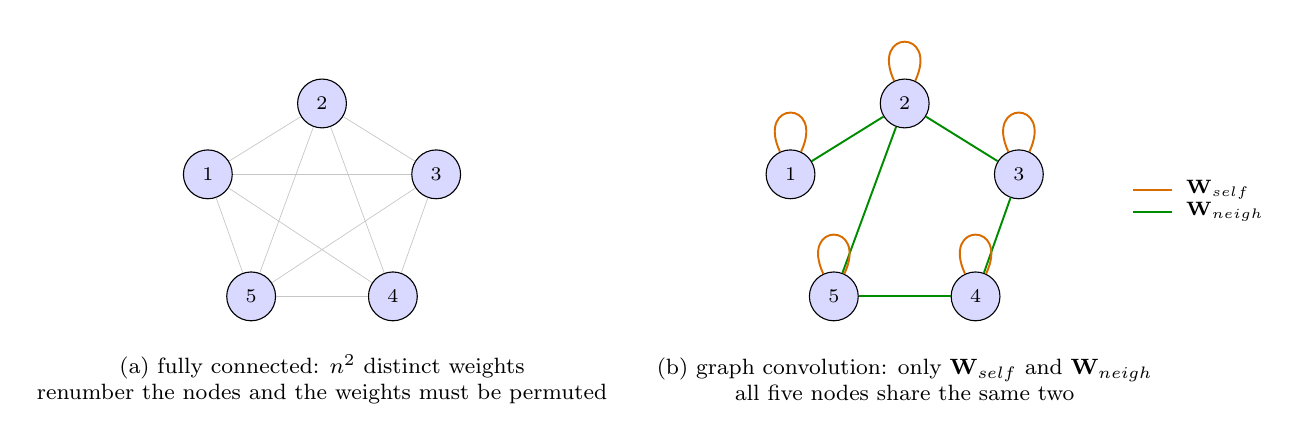
\begin{tikzpicture}[
  every node/.style={font=\small},
  nd/.style={circle, draw, minimum size=0.62cm, inner sep=0pt, font=\scriptsize, fill=blue!15},
  loopstyle/.style={out=115, in=65, looseness=7}
]
\begin{scope}
  \node[nd] (p1) at (0,1.55)    {1};
  \node[nd] (p2) at (1.45,2.45) {2};
  \node[nd] (p3) at (2.9,1.55)  {3};
  \node[nd] (p4) at (2.35,0)    {4};
  \node[nd] (p5) at (0.55,0)    {5};
  \foreach \a/\b in {1/2,1/3,1/4,1/5,2/3,2/4,2/5,3/4,3/5,4/5}
    \draw[gray!45, line width=0.25pt] (p\a) -- (p\b);
  \node[font=\footnotesize, align=center] at (1.45,-1.05)
    {(a) fully connected: $n^2$ distinct weights\\renumber the nodes and the weights must be permuted};
\end{scope}
\begin{scope}[xshift=7.4cm]
  \node[nd] (q1) at (0,1.55)    {1};
  \node[nd] (q2) at (1.45,2.45) {2};
  \node[nd] (q3) at (2.9,1.55)  {3};
  \node[nd] (q4) at (2.35,0)    {4};
  \node[nd] (q5) at (0.55,0)    {5};
  \foreach \a/\b in {1/2,2/3,3/4,4/5,2/5}
    \draw[green!55!black, line width=0.7pt] (q\a) -- (q\b);
  \foreach \v in {1,...,5}
    \draw[orange!85!black, line width=0.7pt] (q\v) to[loopstyle] (q\v);
  \node[font=\footnotesize, align=center] at (1.45,-1.05)
    {(b) graph convolution: only $\mathbf{W}_{\text{self}}$ and $\mathbf{W}_{\text{neigh}}$\\all five nodes share the same two};
  \begin{scope}[shift={(4.35,1.05)}]
    \draw[orange!85!black, line width=0.7pt] (0,0.30) -- (0.5,0.30);
      \node[right, font=\scriptsize] at (0.55,0.30) {$\mathbf{W}_{\text{self}}$};
    \draw[green!55!black,  line width=0.7pt] (0,0.02) -- (0.5,0.02);
      \node[right, font=\scriptsize] at (0.55,0.02) {$\mathbf{W}_{\text{neigh}}$};
  \end{scope}
\end{scope}
\end{tikzpicture}}
\end{center}
\vspace{0.5mm}
{\footnotesize Read the five nodes as five banks and the edges as lending. Flattening the adjacency matrix into a feedforward layer costs $n^{2}$ parameters --- and worse, the parameterisation depends on the \emph{numbering}, which carries no economic content. Graph convolution passes information only along edges that exist, with one $(\mathbf{W}_{\text{self}},\mathbf{W}_{\text{neigh}})$ for every node.}
\vspace{1mm}
\src{Kipf \& Welling (2017). Feng \& Miao, \emph{AI for Economists}, ch.~9, Fig.~9.12.}
\end{frame}

%=============================================================================
\begin{frame}{Permutation Invariance Is an Economic Restriction}
\begin{columns}[T]
\begin{column}{0.54\textwidth}
\small
\[
  \mathbf{h}_v^{(\ell+1)}=\sigma\Bigl(\mathbf{W}_{\text{self}}\mathbf{h}_v^{(\ell)}
  +\!\!\sum_{u\in\mathcal{N}(v)}\!\tfrac{1}{|\mathcal{N}(v)|}\mathbf{W}_{\text{neigh}}\mathbf{h}_u^{(\ell)}+\mathbf{b}\Bigr)
\]
Neighbours come in no particular order, so the aggregation \textbf{must} be order-free --- a sum or a mean. That is not a technical detail. It is the constraint that the answer cannot depend on how the nodes were numbered.
\medskip

And it shows the family resemblance: on a regular grid each pixel's neighbours are a fixed $k$, so the shared weights can be split by position into $w_1,w_2,w_3$. \textbf{Convolution is the special case of this construction on a grid.}
\end{column}
\begin{column}{0.43\textwidth}
\begin{takeawaybox}[title=\textbf{Where you have met this already}]\small
A heterogeneous-agent model requires prices to depend on the distribution \textbf{only through statistics that do not depend on which household is which}.
\medskip
That is the same restriction as permutation invariance --- and it is why a distribution can be fed to a network at all. \textbf{S8 builds on exactly this.}
\end{takeawaybox}
\medskip
\begin{examplebox}\footnotesize
$L$ layers let each node see its $L$-hop neighbourhood. Depth on a graph is \emph{reach}.
\end{examplebox}
\end{column}
\end{columns}
\vspace{1mm}
\src{Feng \& Miao, \emph{AI for Economists}, ch.~9, eq.~(9.33).}
\end{frame}

%=============================================================================
\begin{frame}{Choosing the Constraint}
\vspace{-1mm}
\begin{center}\footnotesize
\begin{tabularx}{\linewidth}{@{}>{\raggedright\arraybackslash}p{1.65cm} >{\raggedright\arraybackslash}p{2.0cm} >{\raggedright\arraybackslash}X >{\raggedright\arraybackslash}p{3.7cm}@{}}
\toprule
\textbf{Data} & \textbf{Architecture} & \textbf{Constraint on $\mathbf{W}$} & \textbf{Typical use in economics} \\
\midrule
tabular & feedforward & none; $\mathbf{W}$ dense & consumption forecasting, \textbf{policy-function approximation}, treatment effects \\
images, spatial & CNN & sparse (local) \emph{and} repeated (shared) & satellite imagery, street view, spatial patterns \\
sequences & RNN, LSTM & one $\mathbf{W}$ across dates; gates make persistence state-dependent & macro time-series forecasting, text sentiment \\
networks, graphs & GNN & sparsity follows adjacency; aggregation order-free & financial-network risk, supply-chain transmission, spillovers \\
\bottomrule
\end{tabularx}
\end{center}
\vspace{0.5mm}
\begin{cautionbox}\footnotesize
The boundaries are not sharp and mixtures are normal --- a CNN makes a feature vector, which then joins tabular variables in a feedforward net. \textbf{When the assumption holds:} fewer parameters, less data, better extrapolation. \textbf{When it fails:} the constraint is simply bias.
\end{cautionbox}
\vspace{0.5mm}
\src{Feng \& Miao, \emph{AI for Economists}, ch.~9, Table~9.8. The course's own use is the first row: 7.B1 approximates a policy function.}
\end{frame}

%=============================================================================
\begin{frame}{What These Architectures Do Not Promise}
\begin{columns}[T]
\begin{column}{0.52\textwidth}
\small
\textbf{The inductive bias may be doing the work, not the depth.} Rolf et al.\ (2021) generate convolutional kernels \textbf{at random}, never train them, and ridge-regress on the resulting features --- matching end-to-end deep training across a range of tasks. What pays is locality and sharing.
\medskip

\textbf{The sequence evidence is mixed.} Paranhos (2025) finds recurrent networks ``competitive but not dominant'' for US inflation; K\i l\i\c{c} (2025) finds threshold and smooth-transition HAR beating LSTM and GRU on realised volatility. Short, noisy macro-financial series are not automatically deep-model territory. The positive case is Barkan et al.\ (2023): a hierarchical RNN following the CPI's own component tree --- \textbf{structure, not scale}.
\end{column}
\begin{column}{0.45\textwidth}
\begin{cautionbox}[title=\textbf{Graphs: an honest reading}]\small
There is as yet \textbf{no mature GNN application in a mainstream economics journal}; the work sits in CS and quantitative-finance preprints.
\medskip
Production-network transmission is still done with structural models and input--output tables, because identification comes from an explicit shock --- and \textbf{the network is endogenous}: whatever made two firms trade may also set how they respond.
\end{cautionbox}
\end{column}
\end{columns}
\vspace{1mm}
\src{Rolf et al.\ (2021), \emph{Nature Communications} (MOSAIKS); Paranhos (2025) and Barkan et al.\ (2023), \emph{IJF}; K\i l\i\c{c} (2025).}
\end{frame}

%=============================================================================
\begin{frame}{Takeaways, and Where the Fourth Constraint Lives}
\begin{columns}[T]
\begin{column}{0.54\textwidth}
\begin{takeawaybox}\small
\begin{itemize}\small\setlength{\itemsep}{1.2mm}
  \item Every architecture here is $\sigma(\mathbf{W}\mathbf{x}+\mathbf{b})$ with a \textbf{restriction on $\mathbf{W}$}: sparse and repeated (CNN), shared across dates (RNN), following the adjacency (GNN).
  \item A restriction is a \textbf{prior about the target function}, not a trick. True, it buys parameters and samples; false, it buys bias.
  \item A CNN is a learned feature extractor plus the feedforward net of 7.A2--7.A3 --- and the feedforward part still holds \textbf{93.1\%} of the parameters.
  \item Order-free aggregation is the same requirement as \textbf{prices depending on a distribution only through index-free statistics}.
\end{itemize}
\end{takeawaybox}
\end{column}
\begin{column}{0.43\textwidth}
\begin{conceptbox}[title=\textbf{Bridge to Block B}]\small
There is a \textbf{fourth} class of constraint, and it is the one economics cares about most: restrict the \textbf{signs} of the weights so the network is monotone, or convex, by construction.
\medskip
That is not a fact about images or sequences. It is a theorem about preferences and value functions, written into the parameterisation --- and it is \textbf{7.B3}.
\end{conceptbox}
\medskip
\begin{examplebox}\footnotesize
\textbf{7.B1} comes first: write a macro model as a loss function, and let the network of 7.A2 approximate its policy.
\end{examplebox}
\end{column}
\end{columns}
\end{frame}

\end{document}
